Zur Müdigkeitserkennung im Zusammenhang mit Auto fahren gibt es verschiedene Methoden, wie sie von Arunasalam et al. \cite{AR20} und Ramzan et al. \cite{RA19} beschrieben werden. Diese lassen sich in drei Hauptkategorien unterteilen:

\begin{itemize}
\item Physiologische Methoden: Hierzu gehören Messungen wie Puls und EEG.
\item Fahrverhaltensbasierte Methoden: Dies umfasst die Analyse des Fahrverhaltens mittles Sensoren am Auto.
\item Verhaltensbasierte Methoden: Hierbei liegt der Fokus auf Beobachtungen von Auge, Gesicht und Kopfbewegungen.
\end{itemize}

Die visuelle Analyse des Verhaltens bietet eine praktikable Lösung, da diese auch vielfältig einsetzbar ist, bepsilesweise auch um Müdugkeit beim Lernen und Arbeiten zu erkennen.

Unser Hauptziel, wie bereits in der Aufgabenstellung erwähnt, besteht darin, eine frühzeitige Warnung auszugeben, wenn eine Person Anzeichen von Müdigkeit zeigt. Wir möchten damit eine Methode entwickeln, um Sekundenschlaf frühzeitig zu verhindern. Dies erfordert die Erkennung von Müdigkeit sowie die Identifizierung von Ablenkung (z. B. wenn eine Person zu lange nicht nach vorne schaut). Die Herausforderung besteht darin, den Zeitpunkt zu bestimmen, ab dem eine Person als müde gelten kann, und objektive Kriterien dafür zu entwickeln. Eine weitere wichtige Herausforderung besteht darin, dass Müdigkeit bei jeder Person unterschiedlich ist und sich visuelle Verhaltensweisen individuell manifestieren. Zum Beispiel variiert die Blinzelrate erheblich von Person zu Person, selbst bei Ruhe (Bentivoglio et al. \cite{BE97} berichtet von 4 bis zu 48 Blinzlern pro Minute).

Unsere Vorgehensweise orientiert sich an Ghodoosian et al. \cite{GH19} und verwendet deren Datensatz als Ausgangspunkt. Wir verarbeiten Videodaten einer Person und extrahieren Landmarks, um quantitative Merkmale zu berechnen. Unsere Schwerpunkte liegen auf den visuellen Eigenschaften des Auges, wobei die Erkennung von Blinzeln eine entscheidende Rolle spielt. Um die Ergebnisse auf individuelle Unterschiede abzustimmen, führen wir eine Kalibrierung durch, die absolute Daten in relative Werte umwandelt. Diese Merkmale werden dann für die Klassifikation von "müde" und "nicht müde" verwendet, woraufhin bei "müde" immer wieder eine Warnung ertönt. Auch ertönt eine Warnung, falls eine Person in Sekundenschlaf verfällt und die Augen über einen längeren Zeitraum geschlossen sind.

\subsection{Gesichtserkennung}
\label{sec:facedetection}

\begin{figure}
    \centering
    \begin{subfigure}{0.3\textwidth}
        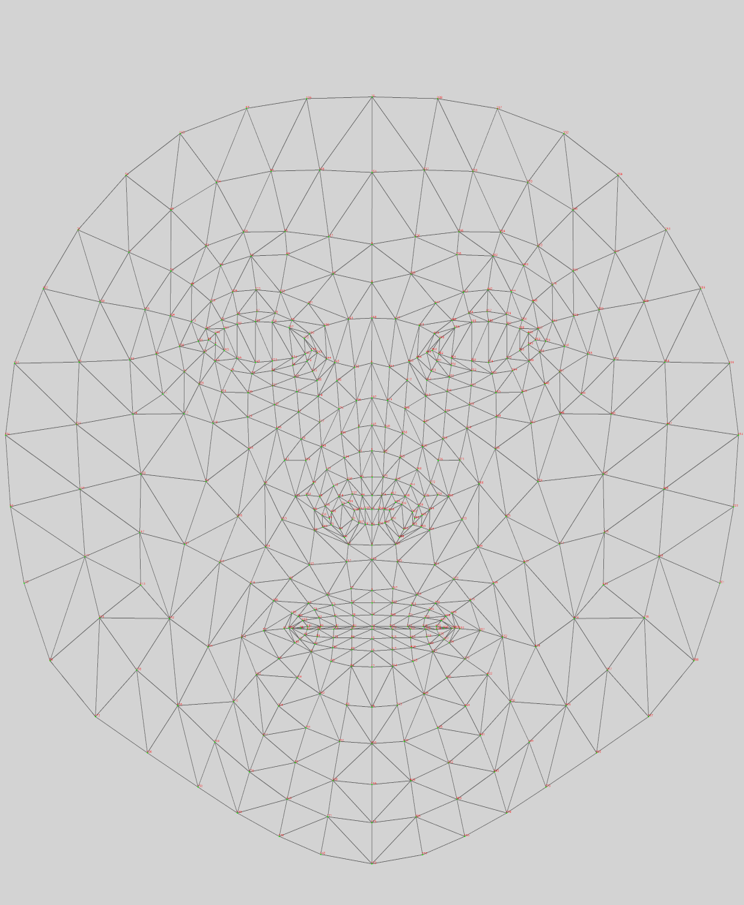
\includegraphics[width=\linewidth]{images/MPFaceMesh1.png}
        \caption{Die Landmarks des Mediapipe Face Mesh mit Nummerierungen.}
        \label{fig:MPFaceMesh1}
    \end{subfigure}
    \hfill
    \begin{subfigure}{0.3\textwidth}
        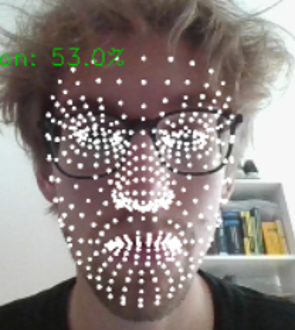
\includegraphics[width=\linewidth]{images/MPFaceMesh2.png}
        \caption{Alle Landmarks des Face Mesh während der Anwendung.}
        \label{fig:MPFaceMesh2}
    \end{subfigure}
    \hfill
    \begin{subfigure}{0.3\textwidth}
        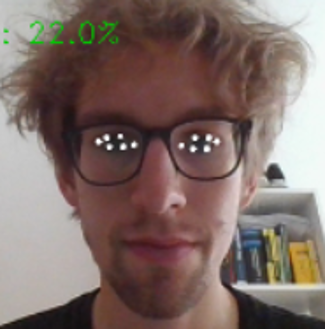
\includegraphics[width=\linewidth]{images/MPFaceMesh3.png}
        \caption{Die Augenlandmarks des Face Mesh zur Berechnung der EAR.}
        \label{fig:MPFaceMesh3}
    \end{subfigure}
    \caption{Prozess der Extraktion der entscheidenden Landmarks für unsere Müdigkeitsdetektion.}
    \label{fig:MPFaceMesh}
\end{figure}

Um verwertbare Daten zu generieren, ist die Echtzeit-Erkennung der Augenstruktur entscheidend, um Blinzler zu identifizieren, was die Grundlage für weitere Analysen bildet. Eine höhere Bildwiederholrate (auch Framerate; Bilder/Sekunde) ermöglicht präzisere Ergebnisse, obwohl die meisten Kameras und Videodaten üblicherweise eine Framerate von etwa 30 Bildern pro Sekunde haben. Es ist von Bedeutung, dass die Framerate durch die Berechnungen des Algorithmus nicht erheblich verlangsamt wird. 

Ein leistungsstarkes und schnelles System dafür ist Mediapipe \cite{LU19}. Das Mediapipe Face Mesh erkennt in Echtzeit 468 3D-Gesichtslandmarks, selbst auf mobilen Geräten, und ermöglicht die Approximation einer 3D-Oberfläche des Gesichts durch maschinelles Lernen. Für unsere Anwendung verwendeten wir Version 0.9.0, um eine Integration mit der Kivy-Bibliothek zu ermöglichen, da eine neuere Version von Mediapipe auf unerklärliche Probleme stieß. In der Version 0.9.0 des Mediapipe Face Mesh bleibt die Grundeinstellung statisch und bewegt sich als Ganzes mit, was jedoch für unsere Untersuchung unzureichend ist. Daher muss die Einstellung "refine" auf "True" gesetzt werden, um 10 zusätzliche Landmarks und Bewegungen innerhalb des Gesichts zu erfassen. Darüber hinaus muss der "static image mode" auf "False" gesetzt werden, um das Face Mesh auf Videos anzuwenden. 

Wir haben auch andere Ansätze für ein Face Mesh evaluiert, darunter den Dlib Face Landmark Detector (Davis E. King \cite{DLIB09}), basierend auf Dalal et al. \cite{DA05}. Im Vergleich zum Mediapipe Face Mesh erzielte dieser jedoch in Bezug auf Genauigkeit schlechtere Ergebnisse und zeigte gelegentlich Aussetzer. Weitere Details dazu finden sich in der Evaluation (siehe \ref{sec:evaluation}).

\subsection{Blinzeldetektion}
\label{sec:blinkdetection}

\begin{figure}
    \centering
    \begin{subfigure}{0.45\textwidth}
        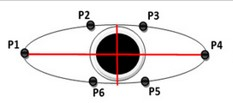
\includegraphics[width=\linewidth]{images/EyeLandmarks.jpg}
        \caption{Die sechs Landmarks von P1 bis zu P6 in ihrer Anordnung am Auge \cite{DE22}}
        \label{fig:eyelandmarks}
    \end{subfigure}
    \hfill
    \begin{subfigure}{0.45\textwidth}
        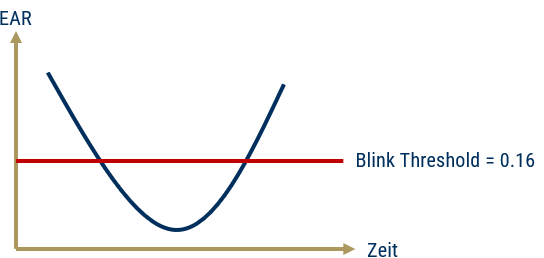
\includegraphics[width=\linewidth]{images/EARCurve.png}
        \caption{Vereinfachte Darstellung eines Blinzelvorgangs und der Auswirkung auf die EAR.}
        \label{fig:earcurve}
    \end{subfigure}
    \caption{Prozess der Berechnung eines Blinzlers über die sechs Augenlandmarks (a) über die EAR Kurve und dem Blink Threshold (b)}
    \label{fig:eyeaspectratio}
\end{figure}

Durch die Berechnung von Landmarks können wir nun das Blinzeln einer Person erkennen. Eine gängige Methode hierfür ist die Berechnung des "Eye Aspect Ratio" (EAR), wie von Soukupova \cite{SO16} präsentiert. Die EAR wird anhand des Auges und sechs Landmarks (P1 bis P6) ermittelt und entspricht dem Verhältnis der vertikalen Öffnung zur horizontalen Öffnung:

\begin{equation}
	\text{EAR} = \frac{{\|P2 - P6\| + \|P3 - P5\|}}{{2\|P1 - P4\|}}
\end{equation}

In dieser Formel repräsentieren P1 bis P6 die Koordinaten der Landmarks, wobei P1 und P4 die äußeren Augenwinkel sind, P2 und P6 die oberen Augenlider und P3 und P5 die unteren Augenlider (Abbildung \ref{fig:eyelandmarks}). Die $ \| \| $ Symbole stellen die euklidische Norm dar, die den Abstand zwischen den Punkten berechnet.

Die EAR ist stets größer, wenn das Auge geöffnet ist, im Vergleich dazu, wenn es geschlossen ist. Allerdings variieren diese Werte erheblich zwischen Personen, wie auch unser eigener Test zeigt, beispielsweise hat Jan-Nicolas Weider einen Wert von x und Mattis Dietrich einen Wert von y (Siehe blabla). Der Durchschnitts-EAR wird über beide Augen berechnet und ermöglicht die kontinuierliche Erfassung dieses Werts für jedes Einzelbild, was weitere Analysen ermöglicht:

\begin{equation}
	\text{Durchschnittliche EAR} = \frac{{\text{EAR}_{\text{linkes Auge}} + \text{EAR}_{\text{rechtes Auge}}}}{2}
\end{equation}

Bei einem Blinzeln zeigt die EAR-Kurve einen typischen Verlauf, der in Abbildung \ref{fig:earcurve} dargestellt ist - sie sinkt zunächst parabelförmig ab und steigt dann wieder an. Ein wichtiger Aspekt ist nun der Schwellenwert, um zu erkennen, ab wann das Auge als "geschlossen" oder "offen" gilt, um ein Blinzeln zu detektieren und seine Dauer zu berechnen. In unseren Selbsttests hat sich vorläufig ein fester Schwellenwert von 0.16 als am besten geeignet erwiesen. Sobald der EAR den Schwellenwert unterschreitet, wird das Auge als geschlossen betrachtet, und wenn er ihn wieder überschreitet, wird der Vorgang als Blinzeln erkannt. Die Blinzelzeit kann anhand der Anzahl der Frames ermittelt werden, in denen der EAR-Wert < 0.16 liegt. Um verschiedene Bildwiederholungsraten auszugleichen, wird die Framerate des Videos verwendet, um einen zeitlichen Wert in Millisekunden zu erhalten. Dies ist entscheidend für die Trainingsphase des Klassifikators und die Anwendbarkeit über verschiedene Bildwiederholungsraten und Geräte hinweg.  Allerdings sollten weitere Untersuchungen zur Verbesserung der Genauigkeit sowie zur Berücksichtigung individueller Unterschiede und möglicher Augenkrankheiten wie Grauer Star oder altersbedingter Verengung der Augen in zukünftigen Arbeiten durchgeführt werden. Eine agile Berechnung der EAR-Schwelle zu Beginn jeder Aufnahme für jede Person könnte eine Möglichkeit sein, wie es von Ghoddoosian et al. \cite{GH19} in ihrem "Blink Retrieval Algorithm" beschrieben wird.

\subsection{Features}
\label{sec:features}

Der nächste Schritt in unserem Verarbeitungsprozess besteht darin, Features zu sammeln. Insbesondere für das Auge stehen verschiedene mögliche Features zur Verfügung, und unterschiedliche Kombinationen können zu besseren Ergebnissen führen, wie von Dreißig et al. \cite{DREI} untersucht wurde. Dreißig et al. hat auch Kopfbewegungen in seine Untersuchungen einbezogen. Aich Ebrahim \cite{EB16} stellt 19 Features vor, die sich ausschließlich auf den Blinzelvorgang beziehen.

Für uns haben sich folgende Features bewährt: die einfache Betrachtung des "Eye Aspect Ratio" (EAR), die durchschnittliche Blinzdauer und der "Percentage of Eye Closure" (PERCLOS) Wert. Der EAR bildet die Grundlage für weitere Features und besitzt auch allein schon Aussagekraft. Wir betrachten die gemittelte EAR über eine Zeitspanne und vergleichen sie mit vorherigen Zeitspannen (Formel). Außerdem analysieren wir die gemittelte EAR über alle Werte > 0.16, um die Werte zu entfernen, wenn das Auge als geschlossen gilt.

Ein weiteres Feature ist die durchschnittliche Blinzdauer. Wenn eine Person müde wird, sollte die Blinzdauer länger sein. Daher speichern wir für jeden Blinzelvorgang die Dauer in Millisekunden und berechnen den Durchschnitt über eine Zeitspanne.
Der PERCLOS-Wert, erstmals von Wierwille et al. \cite{WI94} beschrieben, repräsentiert den Anteil der Zeit in einer Minute, in der die Augen zu mindestens 80 Prozent geschlossen sind. Bei müden Personen wird dieser Wert tendenziell größer. Für eine einfachere Berechnung verwenden wir den PERCLOS-Wert als den Anteil der Zeit in einer Minute, in der der EAR-Wert unterhalb des Schwellenwerts von 0.16 liegt, was darauf hinweist, dass das Auge als geschlossen betrachtet wird.

Die Frage nach der Festlegung der Zeitspanne für diese Berechnungen stellt sich nun als nächstes. Unsere Recherchen ergaben, dass eine Dauer von 60 Sekunden als gängige Spanne angesehen wird, da Werte wie der PERCLOS-Wert pro Minute berechnet werden. Diese Berechnungen erfolgen überlappend, was bedeutet, dass bei jedem neuen Frame neue Werte für die Features generiert werden.

\subsection{Kalibrierung}
\label{sec:calibration}

Eine spezifische Herausforderung, die wir in Anbetracht unserer Aufgabenstellung berücksichtigen müssen, ist die Individualität in Bezug auf die Augenöffnung und das Verhalten bei Müdigkeit. Bei verschiedenen Personen zeigt sich Müdigkeit auf unterschiedliche Weisen: Bei einer Person kann die Blinzeldauer länger werden, während bei einer anderen Person eher die Blinzelhäufigkeit zunimmt. Zusätzlich variiert die EAR bei jeder Person erheblich, wie auch unser Selbsttest bestätigt hat. Daher ist eine Relativierung der Werte unerlässlich.

Zu Beginn jeder Aufzeichnung gehen wir davon aus, dass die Person wach ist, und verwenden die ersten 60 Sekunden, um Referenzwerte für den Wachzustand zu erfassen. Diese Zeitspanne entspricht derjenigen, die für die weiteren Berechnungen verwendet wird. Die für jeden neuen Frame berechneten Werte werden dann in Beziehung zu den Werten des Wachzustands gesetzt. Auf diese Weise erhalten wir immer relative Werte für jedes einzelne Feature.


\subsection{Datensatz}
Bei dem ausgewählten Datensatz zum Trainieren des Klassifikators handelt es sich um den UTA Real-Life Drowsiness Dataset [Quelle]. Der Datensatz stand unglücklicherweise nur zu zwei Drittel zur Verfügung, da auf der offiziellen Seite der Veröffentlichenden technische Probleme zur Zeit der Ausarbeitung vorlagen. In dem verwendeten Datensatz befinden sich jeweils drei Videos von 48 Individuen. Die teilnehmenden Personen wurden so ausgewählt, dass verschiedene Ethnien, Altersgruppen und Geschlechter abgedeckt sind. Weiterhin trug ein Teil der Probanden eine Brille. Die Aufnahmen entstanden jeweils in natürlicher Umgebung mit verschiedenen Perspektiven, Hintergründen und Belichtungsverhältnissen. Pro Person ist ein Video für die Klasse „wach“, „fraglich“ und „müde“ gegeben. Die drei Kategorien ergeben sich, wie in der ABBILDUNG erkenntlich, durch eine Zusammenfassung des offiziellen Karolinska Sleepiness Scale (KSS) [Quelle]. Als „wach“ werden die Stufen eins bis drei betitelt, wobei für „fraglich“ die Stufen 6 und 7 repräsentativ sind. Auf den Zustand „müde“ weisen die Einordnungen in die Stufen acht und neun hin. Die durchschnittliche Länge eines einzelnen Videos beträgt in etwa 10 Minuten, so dass die für die Klassifikation benötigten Featurewerte über einen längeren Zeitraum möglichst genau und fehlerunabhängig ermittelt werden können. 

Bild einfügen

Zu beachten bei der vorliegenden Datengrundlage ist die Tatsache, dass die Videos über verschiedene Dateiformate, Frameraten und Längen verfügen. Einerseits sichert dies die Robustheit des Programms, um mit verschiedener Hardware umgehen zu können, jedoch war andererseits für das automatisierte Einlesen und Featurextrahieren ein Mehraufwand benötigt. Es wurde ein Skript erstellt, welches alle Videos mit den entsprechenden Datenformat aufruft und abspielt und dabei die Extraktion der Features über eine bestimmte Zeit laufen lässt, sodass aus jedem Video relevante Informationen gewonnen werden, alle Werte aus den Videos gleich stark gewichtet sind und zusätzlich kein Video vor einer vollständigen Extraktion aufgrund zu kurzer Aufnahmedauer eines Probanden abbricht.


\subsection{Klassifikation}
\label{sec:classification}

In Bezug auf die drei Videos pro Person setzen wir für jedes Feature den Zustand halbwach und müde in Relation zum Wachzustand und führen daraufhin Klassifikationen basierend auf den relativen Werten durch. Hierbei konzentrieren wir uns auf drei gängige Klassifikatoren und nutzen die Funktionen aus der Bibliothek scikit-learn von Pedregosa et al. \cite{PE11}. Die Ergebnisse werden anhand der folgenden drei Klassifikatoren ausgewertet und verglichen:

\begin{itemize}
\item Logistische Regression: Für zwei Klassen wird die "One-Versus-Rest" (ovr) Multi-Class-Strategie verwendet, während die Strategie für drei Klassen automatisch ausgewählt wird. Das Modell nutzt den 'lbfgs'-Solver und führt bis zu 1000 Iterationen durch, um das Modell zu trainieren.
\item K-Nearest Neighbour mit K=3.
\item Support Vector Machine.
\end{itemize}

Zudem untersuchen wir die Ergebnisse für drei Klassen (müde/fraglich/wach) sowie für zwei Klassen (müde/wach). Wir erwägen auch die Entwicklung eines Scores, haben diese Idee jedoch aufgrund der begrenzten Datenmenge verworfen, da uns lediglich Daten für die Zustände müde, fraglich und wach zur Verfügung standen, jedoch keine weiteren Zwischenwerte.

Die Details zu den Klassifikationsergebnissen werden in der Evaluation genauer analysiert. Für unser Projekt hat sich jedoch der K-Nearest Neighbour als die beste Option erwiesen. Um das System weiter zu verbessern, wäre eine größere Datenmenge von entscheidender Bedeutung. Zusätzlich könnten auch weitere Klassifikatoren in Betracht gezogen werden.



